\chapter{Methodology}

This chapter presents the data filtering process, dataset characteristics, and methodology for quantifying spatial 
openness from interior images and floor plan data. The openness indicators' extractions include the windows ratio, ceilings ratio, floors ratio, 
and walls ratio from interior images, together with tabular based attributes of properties. 
VGAs relies on the floorplan data.
These indicators are used in subsequent temporal, spatial, and correlation analyses.
Figure \ref{fig:method_flow} illustrates the overall methodological framework used in this study, showing the integration of various data sources and analytical approaches to quantify spatial openness.

\begin{figure}[htbp]
    \centering
    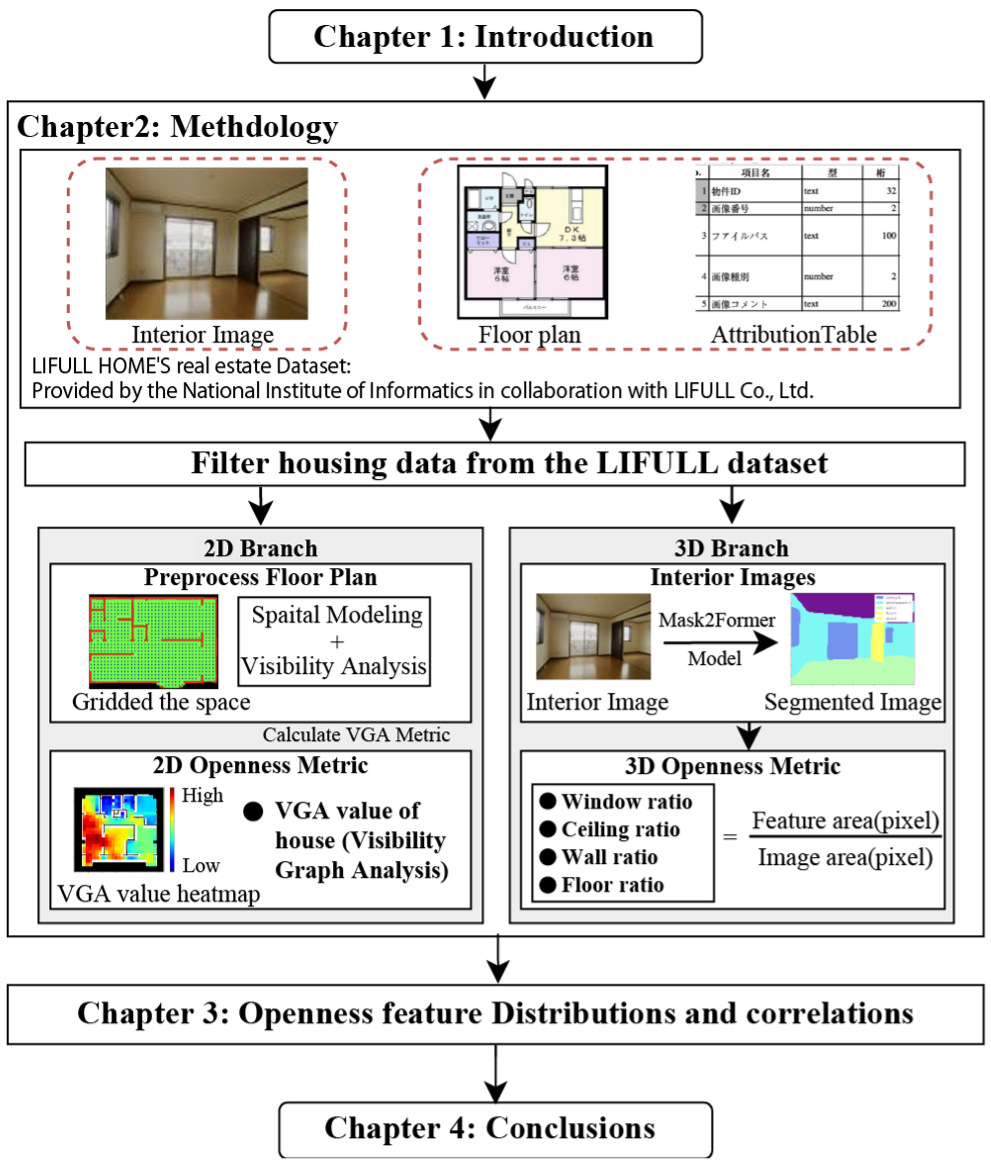
\includegraphics[width=0.9\textwidth]{chapters/plots/method_flow.png}
    \caption{Overall methodological framework showing the integration of 2D floor plan analysis (VGA) and 3D interior image analysis to quantify spatial openness indicators}
    \label{fig:method_flow}
\end{figure}


\section{Overview of Openness }

We consider two types of spatial openness indicators: two-dimensional (2D) openness indicators based 
on the floor plan analysis extracted from floor plans, and three-dimensional (3D) openness indicators based 
on the elevational openness extracted from interior images. Each indicator was calculated using computer 
vision technology from images included in the rental housing big data (LIFULL HOME's dataset). Other 
information such as construction year, location, and property area is included in the attribute table of the 
rental properties.

\section{Dataset Characteristics}

The dataset encompasses multiple categories of spatial openness attributes through interior images, floor plan data, 
and property specifications. Key characteristics include:

\begin{itemize}
    \item \textbf{Temporal Coverage}: Properties spanning from 1960 to present, allowing for longitudinal analysis of 
    spatial design trends
    \item \textbf{Geographic Scope}: Complete coverage of Tokyo's 23 special wards, providing urban-scale spatial 
    analysis capabilities
    \item \textbf{Data Completeness}: Properties filtered for availability of both interior images and floor plan data
\end{itemize}

\subsection{Data Structure and Availability}

The dataset provides multi-modal information for each property:

\begin{itemize}
    \item \textbf{Interior Images}: High-resolution photographs of living spaces, where we focus on the living room, as shown in Figure \ref{fig:exp_inter}.
    \item \textbf{Floor Plans}: Architectural drawings showing spatial layout and room configurations, as shown in Figure \ref{fig:exp_floorplan}.
    \item \textbf{Property Specifications}: Detailed attributes including room size, building age, rent prices, and other basic tabular specs, as exampled in Table \ref{tab:data_sample}.
    addresses.
\end{itemize}

\begin{figure}[htbp]
    \centering
    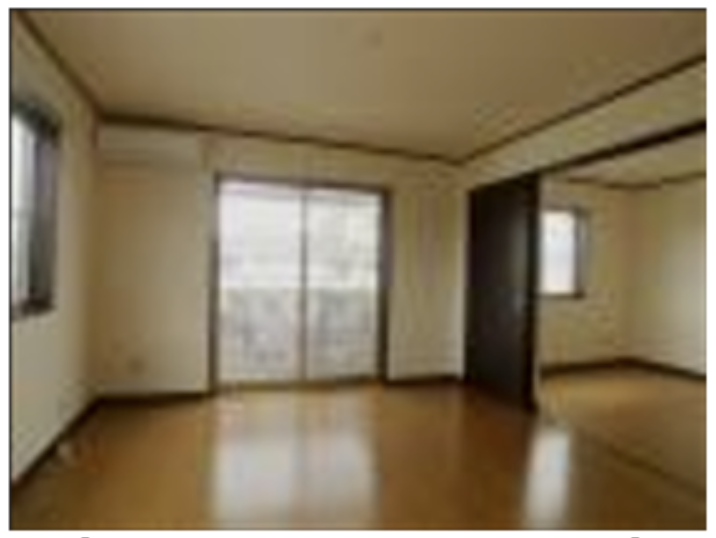
\includegraphics[width=0.7\textwidth]{chapters/plots/exp_inter.png}
    \caption{Example of interior image from the LIFULL dataset.}
    \label{fig:exp_inter}
\end{figure}

\begin{figure}[htbp]
    \centering
    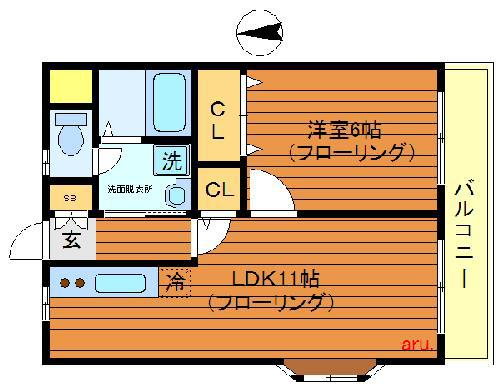
\includegraphics[width=0.8\textwidth]{chapters/plots/exp_floorplan.jpg}
    \caption{Example of floorplan image from the LIFULL dataset.}
    \label{fig:exp_floorplan}
\end{figure}

\begin{table}[h]
\centering
\caption{Sample of LIFULL dataset structure showing key property attributes}
\label{tab:data_sample}
\resizebox{\textwidth}{!}{%
\begin{tabular}{|l|l|l|l|l|l|}
\hline
\textbf{Property ID} & \textbf{Prefecture} & \textbf{City/Ward} & \textbf{...} & \textbf{Building Area} & \textbf{Rent Price} \\
\hline
00026ec12fcea938... & Tokyo & Shibuya & ... & 51.0 & 88000 \\
\hline
00040e134334f56c... & ... & ... & ... & ... & ... \\
\hline
\end{tabular}%
}
\end{table}

\subsection{Multi-Stage Data Filtering Process}

Starting from a raw dataset of over 5 million properties, a systematic multi-stage filtering process is applied to ensure data quality and analytical reliability. The filtering pipeline reduces the dataset to approximately 4,000 final samples suitable for comprehensive openness analysis.

\subsubsection{Initial Data Selection}

The first stage focuses on selecting properties with high-quality visual data:

\begin{itemize}
    \item \textbf{High-Resolution Floor Plans}: Selection of properties with clear, high-resolution floor plan data only, excluding low-resolution variants to ensure adequate spatial detail for VGA analysis and improved semantic segmentation performance
    \item \textbf{Clear Interior Images}: Properties filtered to include only those with clear living room photographs available, ensuring consistent performance when extracting architectural element ratios through semantic segmentation
    \item \textbf{Geographic Constraint}: Properties limited to Tokyo's 23 wards with accurate location data
\end{itemize}

\subsubsection{Property Specification Requirements}

Properties must contain complete tabular specifications including:

\begin{itemize}
    \item \textbf{Location Information}: Accurate geographic coordinates and ward designation within Tokyo's 23 wards
    \item \textbf{Construction Details}: Building construction year, building area, and property type specifications
    \item \textbf{Room Configuration}: Properties must contain room open space area information and at least 1DK room configuration for spatial analysis
    \item \textbf{Essential Attributes}: Complete set of required building-related information for comprehensive analysis
\end{itemize}

\subsubsection{Quality Validation and Final Selection}

The final filtering stage ensures analytical validity:

\begin{itemize}
    \item \textbf{VGA Results Validation}: Properties filtered based on legitimate availability of VGA analysis results from floor plan processing
    \item \textbf{Architectural Element Detection}: Verification that semantic segmentation successfully identifies at least one of the key spatial elements (windows, ceilings, floors, or walls) within interior images
    \item \textbf{Multi-Modal Integration}: Final verification that properties contain all required data modalities (high-resolution floor plans, clear interior images, and complete specifications) for comprehensive openness analysis
\end{itemize}

This systematic filtering process ensures that the final dataset of approximately 4,000 properties maintains high data quality standards while providing sufficient sample size for robust statistical analysis.
The entire filtering process is demonstrated in Figure \ref{fig:data_filtering}.

\section{Sptail Openness Indicators}

Spatial openness is typically expressed through the sense of visual connectivity. 
In residential rental markets, the 3D visual elements displayed in property photographs serve as 
the primary carriers of spatial impression and openness perception for potential tenants. 
The concept of openness in residential spaces encompasses several dimensions, 
with particular emphasis on the following:

\begin{itemize}
    \item \textbf{Visual Connectivity}: The degree to which different areas of a space are visually 
    connected as perceived through interior photographs, which numerically quantified by the VGA analysis.
    
    \item \textbf{Architectural Elements}: The appearance of windows, ceilings, floors, and walls in photos of the living rooms in the LIFULL dataset.
    
\end{itemize}

In the context of rental property advertising, these visual elements become the primary means through which spatial qualities are communicated to potential tenants, making their accurate quantification essential for understanding market dynamics.


%\section{Data Filtering and Cleaning}

In order to effectively extract the required openness features, the data filtering and cleaning pipeline ensures data quality and consistency across the dataset. 
Multiple stages of filtering and validation are applied to maintain analytical reliability. The following sections 
detail the filtering process for interior images, floor plans, and property specifications, which are also illustrated as shown in Figure \ref{fig:data_filtering}.
The details of the methodolgies of how to extract the openness features are demonstrated later after stating the filtering process. 
\begin{figure}[htbp]
    \centering
    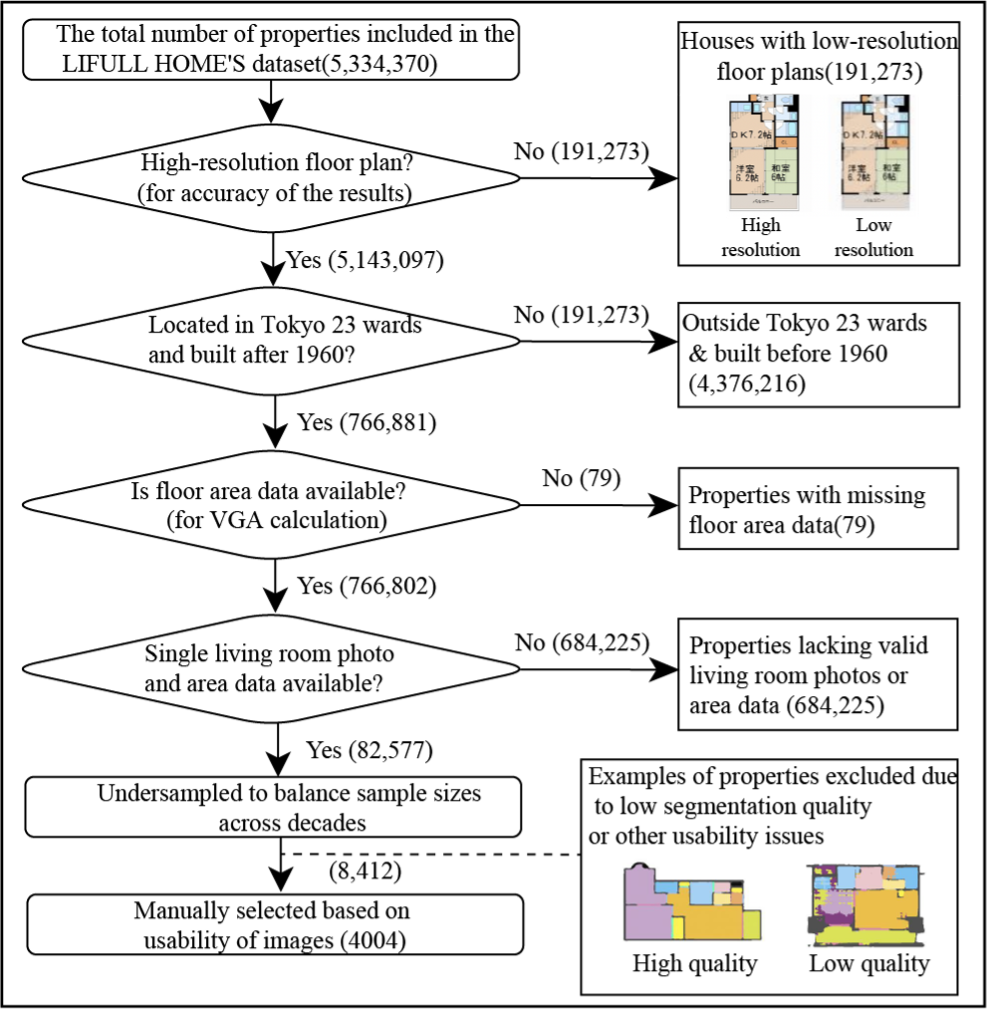
\includegraphics[width=0.9\textwidth]{chapters/plots/data_filtering.png}
    \caption{Data filtering and preprocessing pipeline showing the systematic approach to ensuring data quality and consistency across interior images, floor plans, and property specifications. The flowchart illustrates the multi-stage filtering process from raw data collection to the final integrated dataset.}
    \label{fig:data_filtering}
\end{figure}



\section{2D Openness Indicators}

\subsection{Visibility Graph Analysis (VGA) Methodology}

A key metric for measuring spatial openness is the VGA  (Visibility Graph Analysis) value from floor plans, which 
reflects spatial connectivity. The VGA methodology provides a quantitative approach to assess spatial relationships 
and visual connections within architectural layouts, complementing the impression-based analysis derived from interior photographs.

Traditionally, VGA analysis requires the transformation of optical floor plans into vectorized data formats
 that can be processed using specialized third-party software such as depthmapX \cite{turner2001depthmap}. This conversion process involves:

\begin{itemize}
    \item \textbf{Digitization}: Converting raster floor plan images into vector-based geometric representations
    \item \textbf{Spatial Calibration}: Ensuring accurate scale and dimensional relationships in the vectorized format
    \item \textbf{Boundary Definition}: Precise delineation of walls, openings, and spatial boundaries for visibility calculations
    \item \textbf{Software Processing}: Utilization of specialized tools like depthmapX for comprehensive spatial analysis
\end{itemize}
However, this traditional approach presents significant scalability challenges when applied to large-scale datasets. 
Each floor plan requires individual attention for accurate conversion,
and spatial, calibration, showing a bottleneck that limits its applicability to larger data samples due to the extensive human operations involved.


\subsubsection{Mathematical Definition of VGA}

Corresponding to step 4 in the VGA computational workflow described above, 
the visibility value quantifies the degree of spatial integration and visual 
connectivity within a given floor plan layout. For a discretized spatial grid 
with $N$ points distributed across the open space areas, the visibility graph analysis computes connectivity measures based 
on line-of-sight relationships between grid points.

Mathematically, the visibility value at each point is defined as:
\begin{equation}
\label{eq:vga_definition}
S(i) = \sum_{j=1}^{N} V_{ij}
\end{equation}

where:
\begin{itemize}
    \item $S(i)$ represents the visibility score at grid point $i$
    \item $V_{ij}$ is the visibility indicator function defined as:
    \begin{equation}
    V_{ij} = \begin{cases}
    1 & \text{if point } j \text{ is visible from point } i \\
    0 & \text{otherwise}
    \end{cases}
    \end{equation}
    \item $N$ is the total number of grid points in the open space areas
\end{itemize}

The visibility determination between two points follows the isovist principle \cite{turner2001isovists}, where point $j$ is considered visible from point $i$ if the straight line connecting them does not intersect any wall boundaries identified through the semantic segmentation process.

This computation generates a VGA heatmap $\mathbf{S} = \{S(1), S(2), \ldots, S(N)\}$ representing spatial connectivity throughout the floor plan. From this heatmap, summary statistics including mean ($\mu_S$), standard deviation ($\sigma_S$), and percentiles are extracted as quantitative features characterizing spatial openness for subsequent analysis.


\subsubsection{VGA Computation Process}

To address traditional VGA limitations, we developed a computational workflow using optical floor plan images directly:

\begin{enumerate}
    \item \textbf{Semantic Segmentation}: DeepLab-V3+ model \cite{chen2018encoderdecoderatrousseparableconvolution} fine-tuned to classify walls, bedrooms, and living rooms
    \item \textbf{Boundary Mask Creation}: Generate masks distinguishing walls from open spaces
    \item \textbf{Physical Grid Generation}: Create uniform grid overlay on open space areas
    \item \textbf{Isovist-based Visibility Calculation}: Calculate visibility for each grid point using the isovist method
    \item \textbf{Statistical Extraction}: Extract statistical measures from the resulting heatmap to quantify spatial connectivity
\end{enumerate}
This workflow is demonstrated in Figure \ref{fig:vga_workflow}.

\begin{figure}[H]
    \centering
    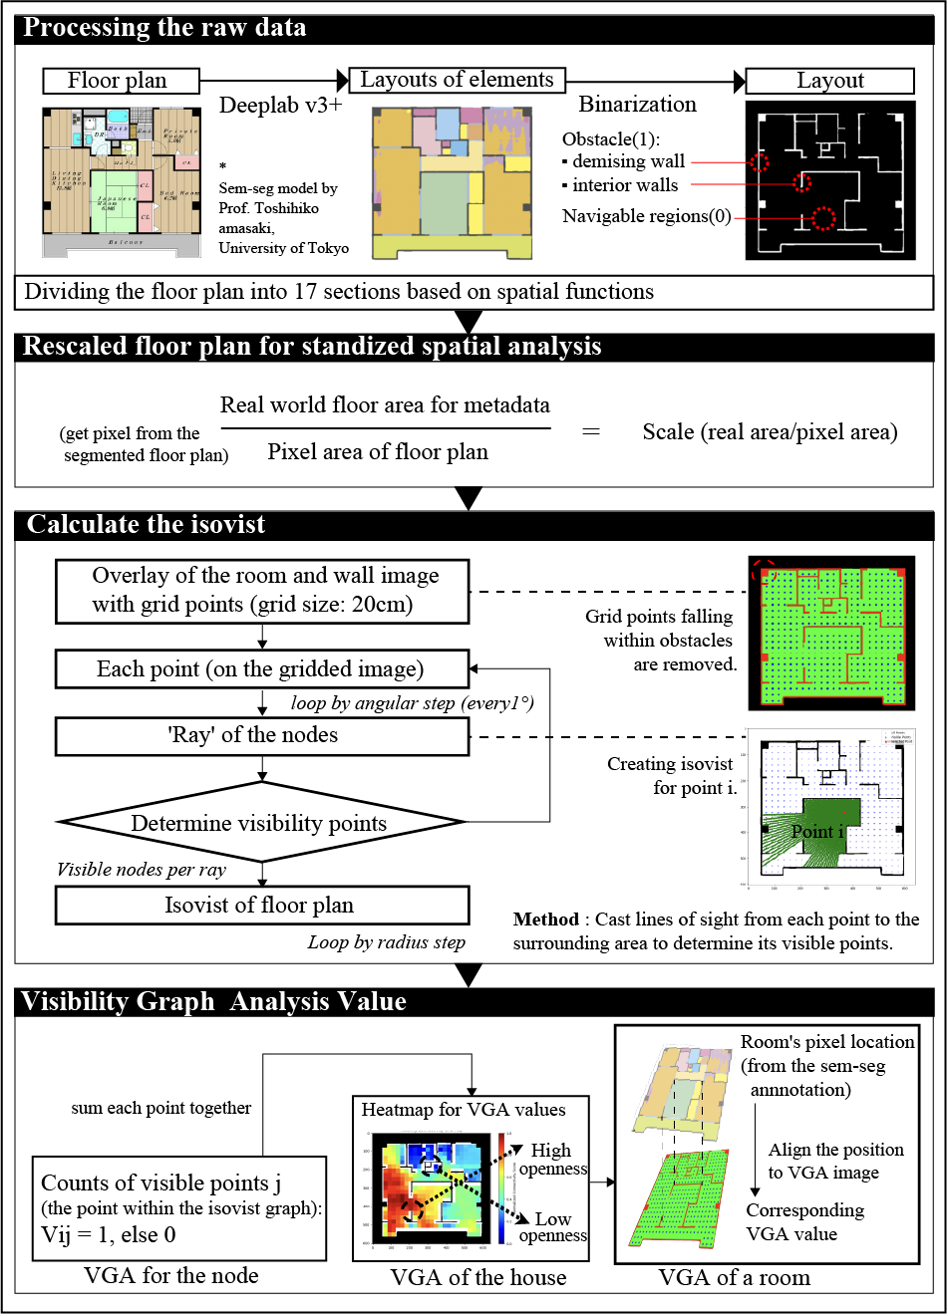
\includegraphics[width=0.9\textwidth]{chapters/plots/vga_workflow.png}
    \caption{VGA computational workflow demonstrating the step-by-step process from semantic segmentation of floor plans to statistical analysis of spatial connectivity.}
    \label{fig:vga_workflow}
\end{figure}



\subsection{3D Openness Indicators}

Beyond VGA analysis, 3D spatial openness is quantified through the analysis of key architectural elements extracted from 
interior images. In our studies, such ratios are calculated from the semantic segmentation results of living room images.

\begin{itemize}
    \item \textbf{Windows Ratio}: Proportion of window area relative to total visible area, indicating natural light 
    access and external connectivity
    \item \textbf{Ceilings Ratio}: Ceiling visibility and height perception contributing to vertical spatial openness
    \item \textbf{Floors Ratio}: Floor area visibility affecting spatial grounding and continuity
    \item \textbf{Walls Ratio}: Wall presence and configuration influencing spatial division and flow
\end{itemize}

These ratios are derived through semantic segmentation techniques applied to interior imagery, providing quantitative 
measures of spatial composition. However, such extraction may have intrinsic uncertainty due to the photo angles and 
standing positions collected from the website, but there is hardly any way to eliminate such issues when requesting 
to use large-scale data from Lifull which is not designed specifically for this study. The methodological details are 
demonstrated in the following sections.

\subsubsection{Segmentation Model}

The semantic segmentation employs a Mask2Former pre-trained model \cite{cheng2022masked}, which is finetuned on the ADE20K dataset \cite{zhou2017scene}
and further optimized for architectural element recognition.

\begin{itemize}
    \item \textbf{Model Selection}: Utilization of state-of-the-art segmentation architectures finetuned on 
    interior image datasets
    \item \textbf{Element Categories}: Classification of pixels into windows, ceilings, floors, walls, and other 
    architectural components
\end{itemize}

\subsubsection{Pixel-wise Classification}

The segmentation process generates pixel-wise masks for each architectural element:

\begin{enumerate}
    \item \textbf{Image Preprocessing}: Standardization of input images for consistent processing, including resizing and batching. 
    \item \textbf{Segmentation Execution}: Application of the trained model to generate semantic masks
    \item \textbf{Post-processing}: recover the original shape and resolutions of the semantic masks to properly calculate the ratios
    \item \textbf{Refinement Process}: Iterative results by ensuring at least one of the four architectural elements (windows, ceilings, floors, walls) appears in the image. 
\end{enumerate}

The above workflow is demonstrated in Figure \ref{fig:segmentation_workflow}.
\begin{figure}[htbp]
    \centering
    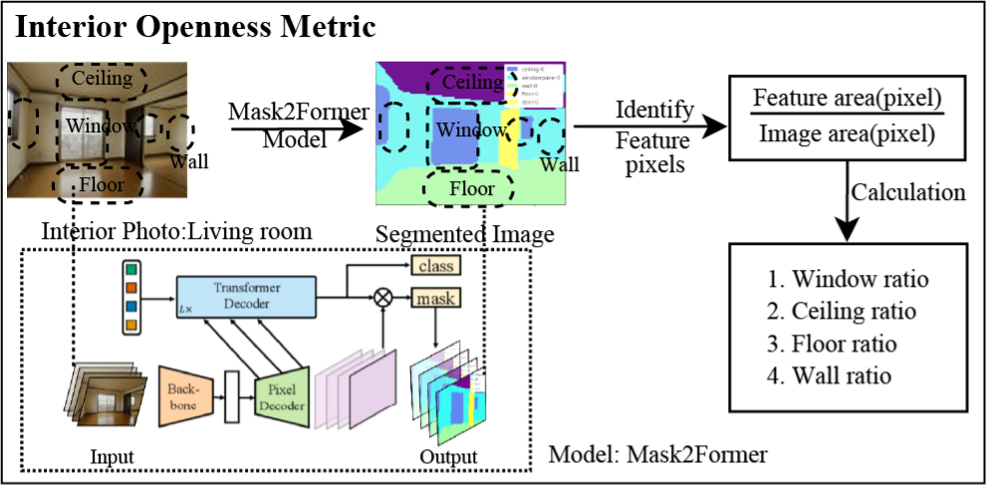
\includegraphics[width=0.95\textwidth]{chapters/plots/inter_semseg.png}
    \caption{Semantic segmentation workflow for architectural element extraction from interior images, showing the process from input image through pixel-wise classification to architectural element ratio calculation.}
    \label{fig:segmentation_workflow}
\end{figure}


\subsubsection{Ratio Calculation}

For each architectural element, the ratio is computed as:

\begin{equation}
    \text{Element Ratio} = \frac{\text{Element Pixel Count}}{\text{Total Image Pixels}}
\end{equation}

This provides a normalized measure of each element's presence within the visual field.

Having established the comprehensive data preparation pipeline and feature extraction methodologies, 
we now transition next chapter for the analytical framework designed to examine the relationship between extracted openness 
features and human perceptions of spatial openness. This analysis encompasses both individual feature 
impacts and their collective influence on openness evaluations.

